\documentclass[crop,tikz]{standalone}

\usepackage{xcolor}
\usepackage{tikz}
\usetikzlibrary{automata, positioning, calc, shapes, arrows, fit}
\newcommand{\mycircle}{\resizebox{!}{0.7em}{\tikz[baseline=(char.base)]{
	\node[shape=circle, fill={rgb:red,0;green,3;blue,8}] (char) {};}}}
\newcommand{\myrectangle}{\resizebox{!}{0.7em}{\tikz[baseline=(char.base)]{
	\node[shape=rectangle, fill={rgb:red,0;green,7;blue,6}] (char) {};}}}
\newcommand{\mydiamond}{\resizebox{!}{0.7em}{\tikz[baseline=(char.base)]{
	\node[shape=diamond, fill={rgb:red,0;green,10;blue,5}] (char) {};}}}

\begin{document}
	
% ============= SOC =============
%\begin{tikzpicture}[node distance = 0.2em and 1em]
%\node[] (a1) {$\mycircle$};
%\node[right = of a1] (b1) {$\succ$};
%\node[right = of b1] (c1) {$\myrectangle$};
%\node[right = of c1] (d1) {$\succ$};
%\node[right = of d1] (e1) {$\mydiamond$};
%
%\node[below = of a1] (a2) {$\mydiamond$};
%\node[right = of a2] (b2) {$\succ$};
%\node[right = of b2] (c2) {$\myrectangle$};
%\node[right = of c2] (d2) {$\succ$};
%\node[right = of d2] (e2) {$\mycircle$};
%
%\node[below = of a2] (a3) {$\myrectangle$};
%\node[right = of a3] (b3) {$\succ$};
%\node[right = of b3] (c3) {$\mycircle$};
%\node[right = of c3] (d3) {$\succ$};
%\node[right = of d3] (e3) {$\mydiamond$};
%\end{tikzpicture}

% ============= SOI =============
%\begin{tikzpicture}[node distance = 0.2em and 1em]
%\node[] (a1) {$\mycircle$};
%\node[right = of a1] (b1) {$\succ$};
%\node[right = of b1] (c1) {$\myrectangle$};
%\node[right = of c1] (d1) {$\succ$};
%\node[right = of d1] (e1) {$\mydiamond$};
%
%\node[below = of a1] (a2) {$\mydiamond$};
%\node[right = of a2] (b2) {$\succ$};
%\node[right = of b2] (c2) {$\myrectangle$};
%
%\node[below = of a2] (a3) {$\myrectangle$};
%\node[right = of a3] (b3) {$\succ$};
%\node[right = of b3] (c3) {$\mycircle$};
%\node[right = of c3] (d3) {$\succ$};
%\node[right = of d3] (e3) {$\mydiamond$};
%\end{tikzpicture}

% ============= TOC =============
%\begin{tikzpicture}[node distance = 0.6em and 1em]
%\node[] (a1) {$\mycircle$};
%\node[right = of a1] (b1) {$\succ$};
%\node[right = of b1] (c1) {$\myrectangle$};
%\node[right = of c1] (d1) {$\succ$};
%\node[right = of d1] (e1) {$\mydiamond$};
%
%\node[below = of a1] (a2) {$\mydiamond$};
%\node[right = of a2] (b2) {$\succ$};
%\node[right = of b2, align = center] (c2) {$\myrectangle{}$\\ $\mycircle{}$};
%
%\node[below = of a2] (a3) {$\myrectangle$};
%\node[right = of a3] (b3) {$\succ$};
%\node[right = of b3] (c3) {$\mycircle$};
%\node[right = of c3] (d3) {$\succ$};
%\node[right = of d3] (e3) {$\mydiamond$};
%\end{tikzpicture}

% ============= TOI =============
%\begin{tikzpicture}[node distance = 0.6em and 1em]
%\node[] (a1) {$\mycircle$};
%\node[right = of a1] (b1) {$\succ$};
%\node[right = of b1] (c1) {$\myrectangle$};
%\node[right = of c1] (d1) {$\succ$};
%\node[right = of d1] (e1) {$\mydiamond$};
%
%\node[below = of a1] (a2) {$\mydiamond$};
%\node[right = of a2] (b2) {$\succ$};
%\node[right = of b2, align = center] (c2) {$\myrectangle{}$\\ $\mycircle{}$};
%
%\node[below = of a2] (a3) {$\myrectangle$};
%\node[right = of a3] (b3) {$\succ$};
%\node[right = of b3] (c3) {$\mycircle$};
%\end{tikzpicture}

% ============= CAT =============
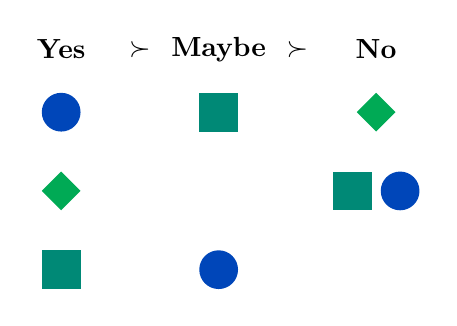
\begin{tikzpicture}[node distance = 0.6em and 1em]
	\node[] (a1) at (0,0) {$\mycircle$};
	\node[] (b1) at (1,0) {};
	\node[] (c1) at (2,0) {$\myrectangle$};
	\node[] (d1) at (3,0) {};
	\node[] (e1) at (4,0) {$\mydiamond$};
	
	\node[] (a0) at (0,0.8) {\bfseries Yes};
	\node[] (b0) at (1,0.8) {$\succ$};
	\node[] (c0) at (2,0.8) {\bfseries Maybe};
	\node[] (d0) at (3,0.8) {$\succ$};
	\node[] (e0) at (4,0.8) {\bfseries No};
	
	\node[] (a2) at (0,-1) {$\mydiamond$};
	\node[] (b2) at (1,-1) {};
	\node[] (c2) at (2,-1) {};
	\node[] (d2) at (3,-1) {};
	\node[] (e2) at (4,-1) {$\myrectangle{}$ $\mycircle{}$};
	
	\node[] (a3) at (0,-2) {$\myrectangle$};
	\node[] (b3) at (1,-2) {};
	\node[] (c3) at (2,-2) {$\mycircle$};
\end{tikzpicture}

\end{document}